\chapter{Diseño e implementación} % Main chapter title
En este capitulo se abordara la descripcion de la arquitectura del sistema, arquitectura del firmware, detalles de los controladores desarrollados para el modulo de comunicaicon y los sensores, desarrollo del hardware y la configuracion de la plataforma IoT. 
\label{Chapter3} % Change X to a consecutive number; for referencing this chapter elsewhere, use \ref{ChapterX}

\definecolor{mygreen}{rgb}{0,0.6,0}
\definecolor{mygray}{rgb}{0.5,0.5,0.5}
\definecolor{mymauve}{rgb}{0.58,0,0.82}

%%%%%%%%%%%%%%%%%%%%%%%%%%%%%%%%%%%%%%%%%%%%%%%%%%%%%%%%%%%%%%%%%%%%%%%%%%%%%
% parámetros para configurar el formato del código en los entornos lstlisting
%%%%%%%%%%%%%%%%%%%%%%%%%%%%%%%%%%%%%%%%%%%%%%%%%%%%%%%%%%%%%%%%%%%%%%%%%%%%%
\lstset{ %
  backgroundcolor=\color{white},   % choose the background color; you must add \usepackage{color} or \usepackage{xcolor}
  basicstyle=\footnotesize,        % the size of the fonts that are used for the code
  breakatwhitespace=false,         % sets if automatic breaks should only happen at whitespace
  breaklines=true,                 % sets automatic line breaking
  captionpos=b,                    % sets the caption-position to bottom
  commentstyle=\color{mygreen},    % comment style
  deletekeywords={...},            % if you want to delete keywords from the given language
  %escapeinside={\%*}{*)},          % if you want to add LaTeX within your code
  %extendedchars=true,              % lets you use non-ASCII characters; for 8-bits encodings only, does not work with UTF-8
  %frame=single,	                % adds a frame around the code
  keepspaces=true,                 % keeps spaces in text, useful for keeping indentation of code (possibly needs columns=flexible)
  keywordstyle=\color{blue},       % keyword style
  language=[ANSI]C,                % the language of the code
  %otherkeywords={*,...},           % if you want to add more keywords to the set
  numbers=left,                    % where to put the line-numbers; possible values are (none, left, right)
  numbersep=5pt,                   % how far the line-numbers are from the code
  numberstyle=\tiny\color{mygray}, % the style that is used for the line-numbers
  rulecolor=\color{black},         % if not set, the frame-color may be changed on line-breaks within not-black text (e.g. comments (green here))
  showspaces=false,                % show spaces everywhere adding particular underscores; it overrides 'showstringspaces'
  showstringspaces=false,          % underline spaces within strings only
  showtabs=false,                  % show tabs within strings adding particular underscores
  stepnumber=1,                    % the step between two line-numbers. If it's 1, each line will be numbered
  stringstyle=\color{mymauve},     % string literal style
  tabsize=2,	                   % sets default tabsize to 2 spaces
  title=\lstname,                  % show the filename of files included with \lstinputlisting; also try caption instead of title
  morecomment=[s]{/*}{*/}
}


%----------------------------------------------------------------------------------------
%	SECTION 1
%----------------------------------------------------------------------------------------
\section{Diagrama de bloques general del sistema}

En la figura \ref{fig:Diagrama general del sistema IoT} se muestra el diagrama en bloques general del sistema donde se describe la arquitectura IoT que consta de tres capas: percepción, red y aplicación.

\begin{figure}[htbp]
	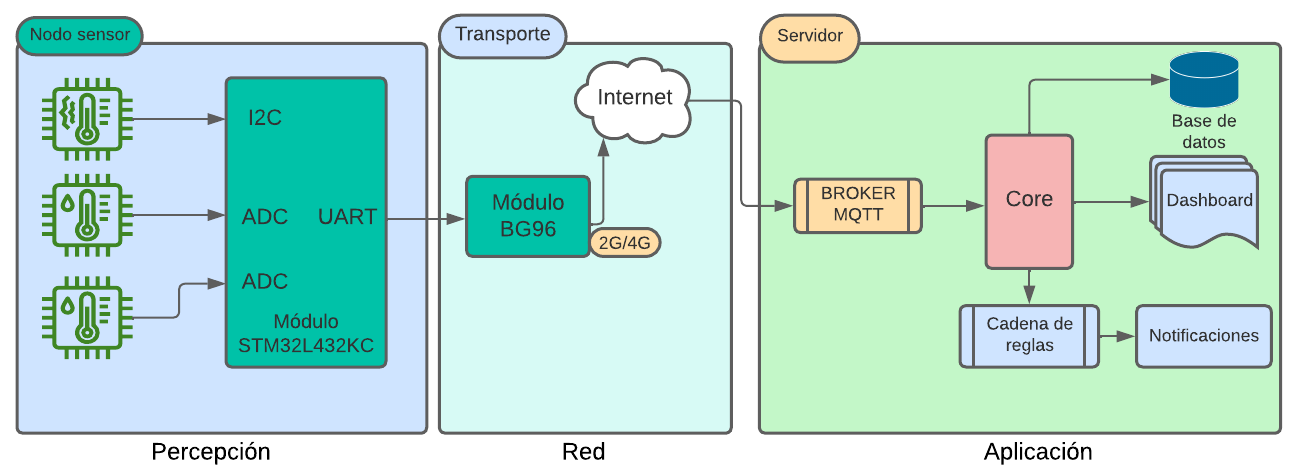
\includegraphics[width=1\textwidth]{./Figures/DiagramaDelSistema.png}
	\caption{Diagrama general del sistema IoT.}
	\label{fig:Diagrama general del sistema IoT}
\end{figure}

En cada una de las capas, se despliegan tecnologias y componentes de hardware y software. A continuación se describe cada una de ellas.

\begin{itemize}
	\item Capa de percepción. En la capa de percepción, los nodos sensores son los encargados de medir variables ambientales, hacer un prepocesamiento y enviarlas a la capa de red. Para su desarrollo se utilizo la placa STM32L432KC que contiene el firmware del sistema,tambien consta de un sensor de humedad y temperatrua ambiente AHT10 que se comunica con la placa de desarrollo mediante el protocolo I2C, sensor de humedad de suelo HL-69 y el sensor de luz UV ML-18 que se comunicacion con el modulo mediante entradas analogicas.
  \item Capa de red. En cuanto a la red, se utilizo un modulo quectel BG96 que puede conectarse a la red 2G, 4G, NB-IoT automaticamente dependiendo del nivel de la red en el lugar de la implementacion del modulo sensor, se comunica con el microcontrolador por comandos AT por puerto UART.
  \item Capa de aplicación. En la capa de aplicacion, se utilizo ThingsBoard como plataforma IoT que nos brinda los microservicios de broker MQTT como puerta de entrada al servidor, base de datos para el almacenamiento, nos brinda la interfaz grafica para la visualizacion de los datos y nos permite gestionar la alarmas del sistema.


\end{itemize}

\section{Arquitectura de firmware}
El desarrollo del firmware fue la tarea mas compleja del proyecto debido a que uno de los objetivos fue lograr 
El firmware fue estructurado en capas como se muestra en la figura se dividio el firmware en capas para facilitar el desarrollo y reducir la complejidad del codigo escritolo separo en capas 
\begin{figure}[htbp]
  \centering
	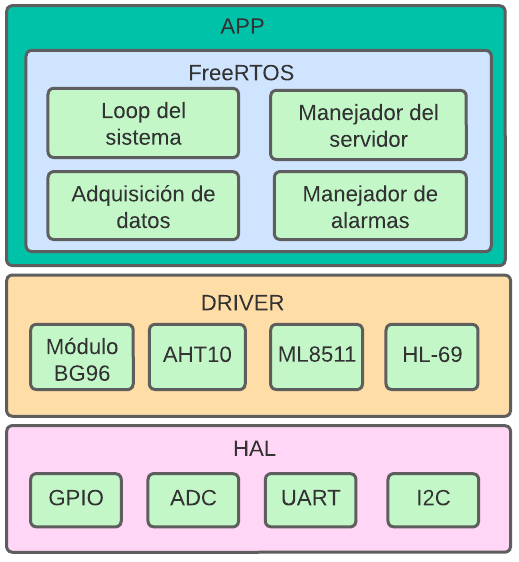
\includegraphics[width=0.7\textwidth]{./Figures/Capas del firmware.png}
	\caption{Capas del firmware.}
	\label{fig:Capas del firmware}
\end{figure}

 La capa Base es la mas baja del sistema y esta compuesta por la libreria HAL de STM, proporciona a las capas superiores la capacidad de interactuar con los perifericos del  microcontrolador STM32L432KC atraves de funciones en lenguaje C
  \begin{itemize}
    \item GPIO: La API proporciona funciones para definir el estado de los pines del microcontrolador.Fueron utilizadas por la capa de APP para el control de los leds de debug del sistema y para el encendido y reset del modulo de comunicacion. Las funciones de esta libreria fue utilizada por la capa de APP para gestionar las entradas y salidas del microcontrolador.
    \item ADC: Proporcionan funciones para la configuracion, lectura y escritura de los pines de microcontroladora senales analogicas. Se utilizaron estas funciones para hacer la lectura de los sensores de humedad de suelo y el sensor de luz UV.
    \item UART: Brinda funciones para la lectura y estritura por el puerto UART del microcontrolador.El firmware utiliza estas funciones para la comunicacion con el modulo BG96.
    \item I2C:Proporciona funciones para la lectura y escritura por protocolo I2C.El driver del sensor de AHT10 utiliza estas funciones para hacer la lectura de los datos.Se utilizaron estas funciones para la lectura de los datos del sensor de AHT10.
    
  \end{itemize}


La capa DRIVERS esta compuesta por los modulos que se desarrollaron para hardware externo al microcontrolador que permiten al microcontrolador enteractuar con hardware externo.Se desarrollaron drivers para el modulo de comunicacion BG96,AHT10,ML18 y HL69
\begin{itemize}
  \item Modulo BG96:Se desarrollo el driver para el modulo BG96, para establecer la comunicacion de este elemento con el microcontrolador a traves del puerto UART.Las funciones mas importantes que proporcionan son
  \begin{itemize}
    \item Estado del modulo.
    \item Descripcion del modulo.
    \item Configuracion APN de la red.
    \item Conexion TCP.
    \item Conexion a broker MQTT.
  \end{itemize}
  \item AHT10: Se desarrollo utilizando la hoja de datos del sensor, proporciona las funciones mas importante inicializacion y lectura de los valores obtenidos por el sensor.
  \item ML18: Se escribio una funcion que permite convertir los datos obtenidos de forma analogica a valores significativos de humedad.
  
\end{itemize}

La capa de APP es la de mayor nivel gerarquico.Se la desarrollo sobre freeRTOS que nos permite hacer un codigo mas escalable.
Se implementaron cuatro tareas
\begin{itemize}
    \item Loop del sistema: Esta tarea es la que nos da la secuencialidad del sistema.
    \item Conexion servidor: Se encarga de manejar la conexion a la red y al broker MQTT.
    \item Adquisicion de datos: Se encarga de hacer la lectura de los sensores.
    \item Manejador de eventos: Esta tarea se encarga de manejar todos lo eventos del sistema.
  \end{itemize}

\section{Desarrollo del firmware}
Para el desarrollo del firmware se utilizo como IDE el IDE oficial de STM cubeIDE 
En la figura se describe el diagrama de flujo de inicializacion del  firmware.

El firmware fue desarrollado sobre freeRTOS, se utilizaron algunas de sus funcionanlidades como queue, semaforos, tareas, interrupciones.En la figura se describe las diferentes tareas que se crearon para el firmware y la comunicacion entre las mismas.



\section{Controladores implementados}






\begin{verbatim}
  \begin{lstlisting}[caption= "un epígrafe descriptivo"]
    las líneas de código irían aquí...
  \end{lstlisting}
  \end{verbatim}

A modo de ejemplo:

\begin{lstlisting}[label=cod:vControl,caption=Pseudocódigo del lazo principal de control.]  % Start your code-block

#define MAX_SENSOR_NUMBER 3
#define MAX_ALARM_NUMBER  6
#define MAX_ACTUATOR_NUMBER 6

uint32_t sensorValue[MAX_SENSOR_NUMBER];		
FunctionalState alarmControl[MAX_ALARM_NUMBER];	//ENABLE or DISABLE
state_t alarmState[MAX_ALARM_NUMBER];						//ON or OFF
state_t actuatorState[MAX_ACTUATOR_NUMBER];			//ON or OFF

void vControl() {

	initGlobalVariables();
	
	period = 500 ms;
		
	while(1) {

		ticks = xTaskGetTickCount();
		
		updateSensors();
		
		updateAlarms();
		
		controlActuators();
		
		vTaskDelayUntil(&ticks, period);
	}
}
\end{lstlisting}



